%! Author = partsjoo
%! Date = 14.04.2023

\newpage


\section{Analysis}

Explain why you chose the levels of generalisations that you did (if you chose ordering, explain why you ordered things the way you did; if you chose intervals, explain how you chose them; if you created a custom hierarchy you can explain the logic behind it).

\subsection{Levels of generalisation}

``id`` is a sensitive attribute because it represents a unique identifier for each individual in the dataset. Protecting this attribute
is critical, as it can directly lead to the re-identification of individuals. Other attributes on their own might not be sufficient to
uniquely identify individuals, but when combined, they can increase the risk of
re-identification. By treating them as quasi-identifiers, I reduce this risk and ensure that the ARX tool considers them when applying
privacy models like k-anonymity and l-diversity~\cite[]{arx}. This approach allows me to apply different levels of privacy protection.

\begin{table}[ht]
  \centering
  \caption{Chosen data transformation types}
  \begin{tabular}{cl}
    \toprule
    \textbf{Sensitive Attributes} & \textbf{Quasi-identifiers} \\
    \midrule
    id                            & Age.at.diagnosis           \\
    & Sex                        \\
    & Native.country             \\
    & Month.first.diagnosis      \\
    & Year.first.diagnosis       \\
    & Vaccination                \\
    & Complicated.phase          \\
    & Critical.phase             \\
    & Last.known.patient.status  \\
    \bottomrule
  \end{tabular}\label{tab:table}
\end{table}


\subsection{Guarantees the privacy models offer}

When analyzing data to anonymize using the ARX tool, I chose to use k-anonymity with k=5 and l-distinct 10-diversity to ensure privacy
and data utility.

K-anonymity is a privacy model that aims to protect individual identities in a dataset by ensuring that each record cannot be uniquely
distinguished from at least k-1 other records~\cite[]{sweeney2002k}. When k-anonymity is set to 5, it means that for any given
combination of quasi
-identifiers (attributes that can be used to identify individuals indirectly) in the dataset, there are at least five records with the same
values. L-distinct diversity is a privacy model that extends k-anonymity by ensuring diversity in sensitive attributes within each group
of records sharing the same quasi-identifiers. This helps protect against attribute disclosure, where an attacker could infer sensitive
information about an individual even if their identity is not revealed~\cite[]{sweeney2002k}. Applying both helps to prevent the re
-identification of individuals in the dataset. Because we had id in out set L-distinct diversity was required by ARX.

A higher value of k-anonymity or L-distinct diversity would provide more privacy, but lead to a significant loss of data utility due to generalisation or suppression
while
lower levels didn't provide enough protection. So I tested with ranges from 2..10 and ended up somwhere in middle of k=5 and l=10. \ac{ico}

\begin{figure}[ht]
  \centering
  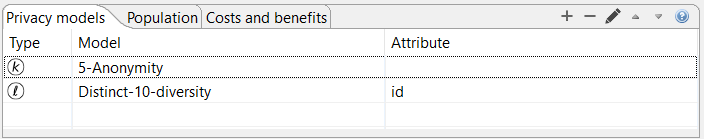
\includegraphics[width=\textwidth]{assets/anon_level}
  \caption{Applied privacy models}
  \label{fig:my_label}
\end{figure}

\subsection{Chosen transformations and levels}

\subsection{Minimal class size}

\subsection{Records were suppressed}

\subsection{Risk of the input data}

\subsection{Risk of the output data}

In about 20\% of our data was consumed which could have been identified and was used for anonymization.
